%===========================================================================================
\subsection{Datasets}


We use the following standard benchmark datasets, largely following the practices in \citet{kuhn2023semantic,lin2023generating}:
\begin{itemize}
    \item CoQA (\datasetcoqa)~\citep{reddy-etal-2019-coqa}, an open-book conversational question answering dataset. 
    We use the development split of \datasetcoqa with 7,983 questions.
    
    \item TriviaQA (\datasettrivia)~\citep{joshi-etal-2017-triviaqa}, a closed-book QA dataset.
    We use the validation split of the \texttt{rc.nocontext} subset of \datasettrivia with 9,960 (de-duplicated) questions. 

    \item Natural Questions (\datasetnqopen)~\citep{kwiatkowski-etal-2019-natural}, a closed-book QA dataset.
    We use the validation split of \datasetnqopen with 3,610 questions.
\end{itemize}
Following~\cite{lin2023generating}, for each experiment we use a random subset of 1,000 questions as the validation set, and the remaining as the test set. 
We report the mean and standard deviation of all evaluation metrics (see~\cref{sec:exp:eval}) on the test set, calculated from 10 random data splittings. 


%===========================================================================================
\subsection{Baselines}
We compare $\methodnamePrompt$ (and $\methodnameNext$) with several recent confidence measures:
\begin{itemize}

    \item $\baselineDegree$, a confidence score based on the degree of similarity graph from~\citet{lin2023generating}.
    Note that this method requires sampling multiple responses, and we set the number of additional generations to $5$.
    We use the ``Entailment'' version as suggested by \citet{lin2023generating}.
    
    \item \baselinePTrue~\citep{kadavath2022language}, which elicits the confidence by asking the LM itself whether its response is correct.
    %This confidence measure uses a prompt to ask the LM itself whether its response is correct, 
    %and computes the confidence from the logits on the options (``correct'' and ``incorrect'') like a classification task. 
    We use the prompt from~\citet{kadavath2022language,lin2023generating}. 

    \item Sequence Likelihood (\baselineNLL): 
    This is the sequence likelihood measure discussed in \cref{eq:confll}, and widely in literature as a confidence score~\cite{lin2023generating,quach2023conformal,huang2024uncertainty} or as a building block for predictive entropy~\citep{kuhn2023semantic,kadavath2022language,malinin2021uncertainty}.
    We include the length-normalized version in \cref{eq:confll:norm}, \baselineNLLNorm, as well.
    
    \item \baselineSAR~\citep{duan2023shifting}:
    It proposes to estimate the relevance of each token as $w_i$ in \cref{eq:main}, with $w_i\propto 1-sim(\predSeq, \predSeq_{-i})$ where $sim$ is similarity measured by an NLI model %represents an external language model that measures the similarity between two sentences 
    and $\predSeq_{-i}$ is the response of interest $\predSeq$ without token $i$.

\end{itemize}
In addition, we also replace the sequence likelihood used in Semantic Entropy (\baselineSE,\citealp{kuhn2023semantic}), which is an \textit{uncertainty}\footnote{See \citet{lin2023generating} for a discussion distinguishing between confidence and uncertainty.} measure, with \methodnamePrompt, and report results in \cref{sec:exp:uncertainty}


%===========================================================================================
\subsection{Language Model and Generation}
For the base LLMs, we include the most popular open LLMs: LLaMA2~\citep{touvron2023llama2}, Mistral~\citep{jiang2023mistral} and Gemma~\citep{team2024gemma}.
We use the 13B version for LLaMA, and the 7B version for Mistral and Gemma due to their improved performance.
Response generation largely follows ~\citet{kuhn2023semantic} with some improvements: The original pipeline often removes content after periods in abbreviations (such as ``Dr.''), so we modified the prompt to ensure each response $\predSeq$ ends with a newline character but keeps contents after punctuations.
%To generate responses, we largely follow the setup of~\citet{kuhn2023semantic} but improve the response cleaning pipeline: The original pipeline often removes content after periods in abbreviations (such as ``Dr.''), so we modified the prompt to ensure each response $\predSeq$ ends with a newline character but keeps contents after punctuations.
Like \citet{kuhn2023semantic}, we focus on the greedily-decoded generation $\predSeq$ for each question and use a temperature of $0.5$ for baselines that require additional response sampling. % more responses.



%===========================================================================================

\def \TabAutoEvalAgreement{
\begin{table}[ht]
\caption{
Agreement with human annotation, on 720 sampled question-response pairs in total.
}
\label{table:main:huamneval}
%\begin{center}
\centering
\begin{small}
   %\resizebox{0.6\columnwidth}{!}{
\begin{tabular}{l|cccc}
\toprule
 Agreement with Human (\%) & \datasetcoqa &  \datasetnqopen & \datasettrivia\\
\midrule
$\Acc_{agree}$ & 98.2 & 91.8 & 98.2\\
$\Acc_{llama2}$ & 97.0 & 86.7 & 95.0\\
$\Acc_{gpt}$ & 94.1 & 85.8 & 96.6 \\
\bottomrule
\end{tabular}
%}
\end{small}
%\end{center}
\end{table}
}
\TabAutoEvalAgreement
\def \TabAUROC{
{
\setlength{\tabcolsep}{3pt}
\begin{table*}%[ht]
%\vspace{-3mm}
\caption{
AUROC of using confidence measures $\Conf$ to predict the accuracy of responses.
Methods not significantly different from the best are in \textbf{bold}. % p=0.01
}
\label{table:main:exp:roc:mlg}
\centering
%\begin{small}
   \resizebox{1.8\columnwidth}{!}{
\begin{tabular}{c|ccccc|cc}
\toprule
& \baselineDegree(E) & \baselinePTrue & \baselineNLL & \baselineNLLNorm & \baselineSAR & \methodnamePrompt & \methodnameNext\\
\midrule
\datasettrivia(llama2) & 81.74$\pm$0.25 & 64.82$\pm$0.18 & 88.19$\pm$0.12 & 87.86$\pm$0.12 & 87.91$\pm$0.13 & \textbf{89.70$\pm$0.19} & \textbf{89.61$\pm$0.18}\\
\datasettrivia(gemma) & 84.00$\pm$0.19 & 81.82$\pm$0.18 & 88.72$\pm$0.11 & 88.11$\pm$0.08 & 88.09$\pm$0.08 & \textbf{89.71$\pm$0.14} & 89.42$\pm$0.11\\
\datasettrivia(mistral) & 81.85$\pm$0.30 & 68.78$\pm$0.28 & 88.81$\pm$0.15 & 88.64$\pm$0.14 & 88.74$\pm$0.13 & \textbf{90.76$\pm$0.18} & \textbf{90.73$\pm$0.15}\\
\datasetcoqa(llama2) & 69.93$\pm$0.57 & 53.64$\pm$0.41 & 69.50$\pm$0.40 & 72.59$\pm$0.44 & 72.78$\pm$0.47 & \textbf{73.34$\pm$0.74} & \textbf{73.36$\pm$0.57}\\
\datasetcoqa(gemma) & 70.03$\pm$0.68 & 55.99$\pm$0.42 & 70.83$\pm$0.46 & 71.96$\pm$0.57 & 72.38$\pm$0.55 & \textbf{73.30$\pm$0.57} & \textbf{73.64$\pm$0.63}\\
\datasetcoqa(mistral) & 69.84$\pm$0.52 & 52.33$\pm$0.42 & 68.97$\pm$0.38 & 70.60$\pm$0.38 & 70.87$\pm$0.41 & \textbf{71.79$\pm$0.75} & \textbf{71.91$\pm$0.63}\\
\datasetnqopen(llama2) & 71.61$\pm$0.51 & 52.51$\pm$0.47 & 66.57$\pm$0.33 & 69.48$\pm$0.50 & 70.43$\pm$0.46 & \textbf{73.73$\pm$0.49} & \textbf{73.54$\pm$0.46}\\
\datasetnqopen(gemma) & 73.32$\pm$0.68 & 63.66$\pm$0.46 & 72.09$\pm$0.65 & 75.81$\pm$0.65 & 75.88$\pm$0.68 & \textbf{77.95$\pm$0.58} & 77.17$\pm$0.65\\
\datasetnqopen(mistral) & 73.03$\pm$0.52 & 54.77$\pm$0.51 & 69.22$\pm$0.53 & 71.06$\pm$0.54 & 72.61$\pm$0.48 & \textbf{76.65$\pm$0.43} & 75.73$\pm$0.68\\
\bottomrule
\end{tabular}
}
%\end{small}
\end{table*}
}}
\TabAUROC

\def \TabAUARC{
{
\setlength{\tabcolsep}{3pt}
\begin{table*}%[ht]
%\vspace{-3mm}
\caption{
AUARC of using confidence measures $\Conf$ to predict the accuracy of responses.
Methods not significantly different from the best are in \textbf{bold}. % p=0.01
}
\label{table:main:exp:arc:mlg}
\centering
   \resizebox{2\columnwidth}{!}{
\begin{tabular}{ccc|ccccc|cc}
\toprule
& Random & Upper Bound & \baselineDegree(E) & \baselinePTrue & \baselineNLL & \baselineNLLNorm & \baselineSAR & \methodnamePrompt & \methodnameNext\\
\midrule
\datasettrivia(llama2) & 82.60$\pm$0.14 & 98.39$\pm$0.03 & 92.84$\pm$0.28 & 87.50$\pm$0.12 & 95.99$\pm$0.06 & 95.95$\pm$0.05 & 95.96$\pm$0.05 & \textbf{96.32$\pm$0.08} & \textbf{96.29$\pm$0.06}\\
\datasettrivia(gemma) & 78.14$\pm$0.13 & 97.41$\pm$0.03 & 91.48$\pm$0.19 & 91.83$\pm$0.11 & 94.61$\pm$0.05 & 94.38$\pm$0.04 & 94.38$\pm$0.04 & \textbf{94.79$\pm$0.04} & 94.65$\pm$0.04\\
\datasettrivia(mistral) & 79.94$\pm$0.12 & 97.84$\pm$0.03 & 91.91$\pm$0.31 & 87.55$\pm$0.13 & 95.27$\pm$0.06 & 95.21$\pm$0.05 & 95.22$\pm$0.05 & \textbf{95.68$\pm$0.09} & \textbf{95.68$\pm$0.07}\\
\datasetcoqa(llama2) & 91.36$\pm$0.17 & 99.62$\pm$0.01 & 94.71$\pm$0.22 & 92.24$\pm$0.18 & 95.69$\pm$0.13 & 96.09$\pm$0.14 & 96.17$\pm$0.14 & \textbf{96.26$\pm$0.18} & \textbf{96.26$\pm$0.16}\\
\datasetcoqa(gemma) & 92.64$\pm$0.14 & 99.72$\pm$0.01 & 95.46$\pm$0.20 & 94.13$\pm$0.15 & 96.54$\pm$0.10 & 96.63$\pm$0.11 & 96.68$\pm$0.11 & \textbf{96.85$\pm$0.11} & \textbf{96.90$\pm$0.13}\\
\datasetcoqa(mistral) & 92.04$\pm$0.14 & 99.67$\pm$0.01 & 95.09$\pm$0.33 & 92.62$\pm$0.16 & 95.92$\pm$0.10 & 96.13$\pm$0.11 & 96.22$\pm$0.10 & \textbf{96.37$\pm$0.13} & \textbf{96.38$\pm$0.12}\\
\datasetnqopen(llama2) & 56.49$\pm$0.68 & 88.74$\pm$0.39 & 70.59$\pm$1.27 & 57.68$\pm$0.68 & 70.51$\pm$0.76 & 71.01$\pm$0.81 & 71.97$\pm$0.80 & \textbf{73.46$\pm$0.66} & \textbf{73.31$\pm$0.87}\\
\datasetnqopen(gemma) & 47.16$\pm$0.65 & 82.59$\pm$0.49 & 62.96$\pm$0.94 & 57.30$\pm$0.67 & 65.78$\pm$0.95 & 66.41$\pm$0.92 & 67.02$\pm$0.93 & \textbf{67.78$\pm$1.07} & 66.89$\pm$1.03\\
\datasetnqopen(mistral) & 52.90$\pm$0.74 & 86.57$\pm$0.47 & 67.48$\pm$1.00 & 56.47$\pm$0.93 & 69.15$\pm$0.82 & 69.27$\pm$0.72 & 70.62$\pm$0.65 & \textbf{72.25$\pm$0.74} & 71.85$\pm$0.69\\
\bottomrule
\end{tabular}
}
\end{table*}
}}
\TabAUARC

\subsection{Evaluation}\label{sec:exp:eval}

For an effective confidence measure, low confidence should correlate with a higher probability of incorrect generation.
To assess the quality of confidence measures, we adhere to established methodologies \citep{kuhn2023semantic,Band2022BenchmarkingBD}.
This involves utilizing them to predict the correctness of a generation and calculating the Area Under the Receiver Operating Characteristic curve (\textbf{AUROC}) for this prediction task.
Formally, let $\Acc_{i}$ represent the indicator function $\mathbbm{1}\{\predSeq_i \text{ correctly answers } x_i\}$. 
We compute the AUROC using the confidence measure $\Conf(x_\cdot, \predSeq_\cdot)$ to predict $\Acc_\cdot$. 
This approach allows us to systematically evaluate how well the confidence measures distinguish between correct and incorrect responses across multiple samples.

In addition to AUROC, following~\citet{lin2023generating}, we also report Area Under Accuracy-Rejection Curve (\textbf{AUARC})~\citep{auarc}.
The Accuracy-Rejection Curve (ARC) computes the average the accuracy when a subset of samples is rejected based on $\Conf$. 
As we exclude more low-confidence samples, the accuracy of the remaining samples should increase. 
The \textit{upper bound} is achieved by predicting only the correct $\predSeq$ (i.e. set $\Conf$ to accuracy), and the AUARC of a \textit{random} predictor is equal to the base accuracy without rejection.


\textbf{Correctness of Generations}:
A critical requirement for computing AUROC or AUARC is a reliable $\Acc_{i}$, the accuracy of each response. 
%the evaluation of confidence measures using AUROC or AUARC is that we need to know $\Acc_{i}$, the accuracy of each response. 
This is a unique challenge in UQ for NLG, and deserves separate research. %, because we do not have such correctness labels like in usual classification tasks.
Prior work typically relies on lexical similarity measures such as ROUGE~\citep{kuhn2023semantic,quach2023conformal} or BLEU~\citep{huang2024uncertainty}.
\citet{lin2023generating} uses \texttt{gpt-3.5} to evaluate the correctness of each response given a reference answer\footnote{The original paper uses \texttt{gpt-3.5-turbo-0301} which is no longer accessible.}, and considers anything with a rating above 70\% as correct.
Inspired by~\cite{lin2023generating}, we use the agreement of both \LLaMATwoName and \GPTName's evaluations as $\Acc$ (More details are in \cref{appendix:autoeval}).
As shown in \cref{table:main:huamneval}, this notably improves the correctness evaluation and thus the reliability of AUROC/AUARC.
We include the results using $\Acc_{llama2}$ in the \cref{appendix:llama2_acc} since $\Acc_{agree}$ and $\Acc_{gpt}$ may not remain reproducible in the future.

% We randomly sample 720 question and response pairs, label the correctness of the responses, and then pick thresholds for \LLaMATwoName and \texttt{gpt-3.5-turbo-0125} that maximizes their agreement with the human annotations.
% We found that by keeping only the agreement between \LLaMATwoName and \GPTName, we can notably improve the correctness evaluation and thus the reliability of AUROC/AUARC, as shown in \cref{table:main:huamneval} (More details are in \cref{appendix:autoeval}).
% We refer to the correctness label as $\Acc_{gpt}$, $\Acc_{llama2}$ and $\Acc_{agree}$. All results in the main paper were computed using $\Acc_{agree}$.
% We include the results using $\Acc_{llama2}$ in the \cref{appendix:llama2_acc} since $\Acc_{agree}$ and $\Acc_{gpt}$ may not remain reproducible in the future.



%===========================================================================================
\subsection{Results}\label{sec:exp:result}
\cref{table:main:exp:roc:mlg} presents the AUROC of different confidence measures.
Clearly, all the confidence baselines consistently detect good $\predSeq$ over bad ones, but \methodname outperforms baselines.
Similar results are observed for AUARC in \cref{table:main:exp:arc:mlg} as well: As the LMs have good base accuracy (from the ``Random'' column) for \datasetcoqa and \datasettrivia, the gap between different confidence measures is relatively small, but generally significant.
In particular, among likelihood-based methods, it is sometimes confusing whether normalized or unnormalized likelihood should be used~\citep{kuhn2023semantic,malinin2021uncertainty}, and 
\baselineSAR does not always outperform the better of the two.
However, \methodname consistently outperforms all three.
Thanks to the additional sampling, \baselineDegree performs quite well, especially if we further increase the temperature of the base LM (see Appendix), but in practice it could significantly increase the computation cost as it requires $m$ additional generations and $O(m^2)$ similarity comparisons.
Finally, after the head selection process, the difference between \methodnamePrompt and \methodnameNext is small, but still extremely significant if we perform a pooled test. %paired t-test.
The observed similar performance is because chosen attention heads exhibit highly correlated patterns (see \cref{sec:exp:deeperattn}).
We recommend \methodnamePrompt over \methodnameNext as they share similar overhead (close to none) but the attention-eliciting prompt is more structured compared with the more arbitrary prompt used to generate $\predSeq$, and therefore the ``good'' heads are likely to be more stable.



%===========================================================================================
\def \TabUQ{
{
\setlength{\tabcolsep}{3pt}
\begin{table}%[ht]
\caption{
AUROC of using variants of Semantic Entropy to predict the accuracy of responses.
%Methods not significantly different from the best are in \textbf{bold}. % p=0.01
\methodSEAttn significantly improves the original version based on vanilla sequence likelihoods.
}
\label{table:main:exp:roc:uq}
\centering
%\begin{small}
   \resizebox{.9\columnwidth}{!}{
\begin{tabular}{c|cc|c}
\toprule
  & \baselineSENorm & \baselineSE & \methodSEAttn\\
\midrule
\datasettrivia(llama2) & 89.88$\pm$0.11 & 89.33$\pm$0.12 & \textbf{90.50$\pm$0.12}\\
\datasettrivia(gemma) & 90.33$\pm$0.10 & 90.02$\pm$0.12 & \textbf{90.75$\pm$0.13}\\
\datasettrivia(mistral) & 90.35$\pm$0.12 & 89.78$\pm$0.15 & \textbf{91.13$\pm$0.13}\\
\datasetcoqa(llama2) & \textbf{75.26$\pm$0.33} & 72.50$\pm$0.34 & \textbf{75.58$\pm$0.51}\\
\datasetcoqa(gemma) & \textbf{74.81$\pm$0.48} & 72.95$\pm$0.48 & \textbf{75.08$\pm$0.50}\\
\datasetcoqa(mistral) & 74.06$\pm$0.41 & 71.54$\pm$0.32 & \textbf{74.56$\pm$0.51}\\
\datasetnqopen(llama2) & 74.13$\pm$0.51 & 69.62$\pm$0.38 & \textbf{76.33$\pm$0.50}\\
\datasetnqopen(gemma) & 77.93$\pm$0.58 & 73.67$\pm$0.77 & \textbf{79.50$\pm$0.52}\\
\datasetnqopen(mistral) & 75.71$\pm$0.40 & 71.85$\pm$0.49 & \textbf{78.66$\pm$0.35}\\
\bottomrule
\end{tabular}
}
\end{table}
}}
\TabUQ
\subsection{Improving Uncertainty Measures}\label{sec:exp:uncertainty}
%\vspace{-1mm}
As noted earlier, sequence likelihood is widely used in entropy computation, which is used as an uncertainty measure for NLG.
Semantic Entropy~\citep{kuhn2023semantic} is a state-of-the-art uncertainty measure that groups sampled generations into semantic sets and computes the entropy over these sets.
In doing so, it uses sequence likelihood (sometimes normalized). We simply replace it with \methodnamePrompt to create a new uncertainty measure, \methodSEAttn.
The comparison is shown in \cref{table:main:exp:roc:uq}.
\methodSEAttn consistently outperforms either the normalized or the unnormalized version of $\baselineSE$, showing potential in replacing sequence likelihood in other domains such as conformal NLG~\cite{quach2023conformal}.
%\vspace{-1mm}

%===========================================================================================
%\subsection{A Closer Look into the Attention Values}\label{sec:exp:deeperattn}
\subsection{Is the Improvement a Fluke?}\label{sec:exp:deeperattn}


\def \FigAttnCorr{
\begin{figure}[ht]
\centering
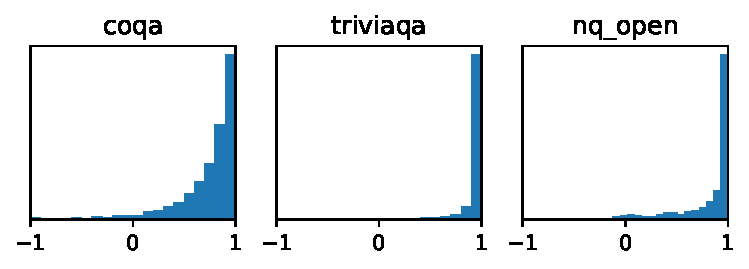
\includegraphics[width=0.45\textwidth]{Figures/attncorr_variants_llama2.pdf}
\caption{
Histogram of the correlation between attentions from \methodnamePrompt and \methodnameNext (top 10 heads' average).
We keep only generations with more than 2 tokens.
For most responses, the chosen heads' attentions are highly correlated, suggesting that both methods focus on the same tokens, as exemplified in \cref{fig:main:case}.
}
% \vspace{-5mm}
\label{fig:attncorr}
\end{figure}
}
\FigAttnCorr

Despite not using an explicit attention-eliciting prompt, \methodnameNext performs close to \methodnamePrompt, outperforming baselines significantly.
It is reasonable to then worry that the improvement is just the result of black-box data-mining by the head-selection step in \cref{sec:method:headchoice}.
This section presents evidence that \methodname most likely identifies meaningful concepts.

\cref{fig:attncorr} shows the correlation between the $w_i$ vectors used for \methodnamePrompt and \methodnameNext---which is almost always positive and usually close to 1. 
As the prompts used to induce these attention weights are quite different, such agreement could be taken as preliminary evidence that these weights are ``meaningful'' and less likely to be purely the results of two independent black-box ``fitting'' processes.


\begin{figure}[ht]
\begin{small}
  \begin{framed}
\textit{Question 1:} how early did he want to get there?\\
\textit{Response 1:} \attnplus{an hour before} the time\\
\textit{Question 2:} What does Barwell think of him?\\
\textit{Response 2:} \attnplus{he} is \attnplus{not fit} to be his guard\attnplus{ian}\\
\textit{Question 3:} who is Susan Boyle?\\
\textit{Response 3:} \attnplus{Susan} Bo\attnplus{yle is a Scottish singer who} became \attnplus{famous} after appearing on the TV show "Britain\attnplus{'}s Got Talent" in \attnplus{2}009\attnplus{.}
  \end{framed}
  \end{small}
\caption{
Tokens whose attention is increased are \attnplus{marked} (others decreased).
As expected, such re-weighting are not always interpretable, but help locating the more relevant tokens in general.
}\label{fig:main:case}
\end{figure}
\cref{fig:main:case} shows a few examples of the induced attention weights, illustrating how \methodname makes the confidence measure more focused on important tokens.
Given the nature of soft attention, despite the fact that $w_i$ chosen by \cref{sec:method} generally identifies the important tokens and improves upon vanilla sequence likelihood, it is still sometimes difficult to interpret why each token is under/over-weighted. 
This brings us to an important distinction between \methodname and how attention is typically used in research on the interpretability of deep (language) models such as \cite{10.1145/3357384.3358028,biju-etal-2022-input}: We leverage such soft attention values mostly on an aggregate level to improve the confidence scores, yet to achieve interpretability via them is often more difficult.
For interpretability reasons, a future research direction might be to directly use natural language to identify such tokens. 
For example, one might directly ask the LM to list the important entities with respect to a question.
The challenge, then, transfers to identifying the actual tokens implied by the natural language output listing important entities in the original $\predSeq$.

Finally, if the attention weights are actually focusing on the important concepts as intended, one might expect that they should transfer \textit{between datasets} and be more robust to distribution shifts.
In \cref{table:main:exp:roc:coqa_transfer}, we select heads based on validation sets from \datasetcoqa and apply them on the other two datasets, which are quite different from \datasetcoqa (e.g. in the format of questions).
\methodnamePrompt still provides consistent performance boost, while \methodnameNext sometimes lags behind \baselineNLLNorm.
This suggests both the prompt and the head selection step increase the weights on the more relevant tokens.


\def \TabCoqaTransfer{
{
\setlength{\tabcolsep}{3pt}
\begin{table}%[ht]
\caption{
AUROC using heads picked from \datasetcoqa.
Despite the big distribution shift from \datasetcoqa to \datasetnqopen/\datasettrivia, the heads chosen on \datasetcoqa still provides attention weights that significantly improves the AUROC.
}
\label{table:main:exp:roc:coqa_transfer}
\centering
%\begin{small}
   \resizebox{.9\columnwidth}{!}{
\begin{tabular}{c|ccc}
\toprule
 & \baselineNLLNorm & \methodnamePrompt & \methodnameNext\\
\midrule
\datasettrivia(llama2) & 87.86$\pm$0.12 & \textbf{88.59$\pm$0.85} & 88.37$\pm$0.87\\
\datasettrivia(gemma) & 88.11$\pm$0.08 & \textbf{89.03$\pm$0.61} & 87.43$\pm$0.94\\
\datasettrivia(mistral) & 88.64$\pm$0.14 & \textbf{89.70$\pm$1.43} & 88.46$\pm$1.93\\
\datasetnqopen(llama2) & 69.48$\pm$0.50 & \textbf{70.94$\pm$1.66} & 70.10$\pm$2.09\\
\datasetnqopen(gemma) & 75.81$\pm$0.65 & \textbf{77.21$\pm$1.06} & 74.99$\pm$1.30\\
\datasetnqopen(mistral) & \textbf{71.06$\pm$0.54} & \textbf{72.71$\pm$3.32} & \textbf{72.27$\pm$2.72}\\
\bottomrule
\end{tabular}
}
\end{table}
}
}
\TabCoqaTransfer


%===========================================================================================
\subsection{Ablation: Choice of Attention Heads}
\def \TabHeadChoice{
{
\setlength{\tabcolsep}{3pt}
\begin{table}%[ht]
%\vspace{-3mm}
\caption{
AUROC of different choice of heads.
Using all heads, heads from last layer, or the best head are generally better than equal-weighted (\baselineNLLNorm) but worse than using the best 10 heads (\methodname).
}
\label{table:main:exp:roc:head_choice}
\centering
%\begin{small}
   \resizebox{1\columnwidth}{!}{
\begin{tabular}{c|cccc|c}
\toprule
  & \baselineNLLNorm & \methodname(best) & \methodname(all) & \methodname(last) & \methodname ($k=10$)\\
\midrule
triviaqa(llama2) & 87.86$\pm$0.12 & 89.26$\pm$0.48 & 87.75$\pm$0.12 & 87.17$\pm$0.12 & \textbf{89.70$\pm$0.19}\\
triviaqa(gemma) & 88.11$\pm$0.08 & 89.32$\pm$0.31 & 88.08$\pm$0.08 & 88.35$\pm$0.07 & \textbf{89.71$\pm$0.14}\\
triviaqa(mistral) & 88.64$\pm$0.14 & 90.46$\pm$0.27 & 89.18$\pm$0.12 & 88.41$\pm$0.14 & \textbf{90.76$\pm$0.18}\\
coqa(llama2) & 72.59$\pm$0.44 & 72.46$\pm$1.25 & \textbf{73.14$\pm$0.49} & \textbf{73.09$\pm$0.49} & \textbf{73.34$\pm$0.74}\\
coqa(gemma) & 71.96$\pm$0.57 & 72.34$\pm$1.00 & 72.79$\pm$0.59 & 72.01$\pm$0.58 & \textbf{73.30$\pm$0.57}\\
coqa(mistral) & 70.60$\pm$0.38 & 70.86$\pm$1.07 & \textbf{71.35$\pm$0.38} & \textbf{71.66$\pm$0.38} & \textbf{71.79$\pm$0.75}\\
nq(llama2) & 69.48$\pm$0.50 & \textbf{73.23$\pm$0.77} & 68.72$\pm$0.51 & 67.70$\pm$0.55 & \textbf{73.73$\pm$0.49}\\
nq(gemma) & 75.81$\pm$0.65 & \textbf{77.45$\pm$0.89} & 76.37$\pm$0.65 & 76.76$\pm$0.69 & \textbf{77.95$\pm$0.58}\\
nq(mistral) & 71.06$\pm$0.54 & \textbf{76.41$\pm$0.50} & 70.83$\pm$0.57 & 69.73$\pm$0.60 & \textbf{76.65$\pm$0.43}\\
\bottomrule
\end{tabular}
}
%\end{small}
\end{table}
}}
%\TabHeadChoice

\def \FigHeadChoice{
\begin{figure}[ht]
\centering
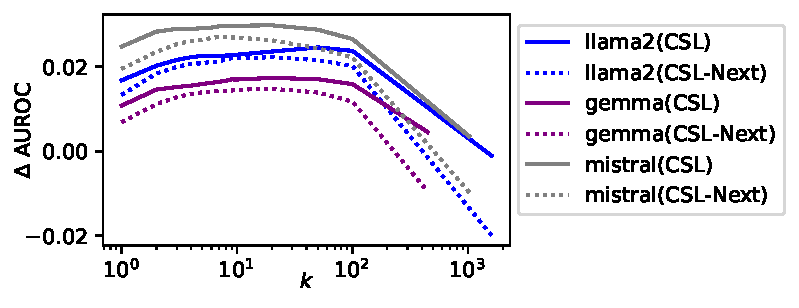
\includegraphics[width=0.48\textwidth]{Figures/num_heads.pdf}
% \vspace{-7mm}
\caption{
AUROC gain compared with \baselineNLLNorm for different $k$ (number of attention heads to keep), from 1 to all heads.
%Solid lines represent \methodnamePrompt and dotted lines, \methodnameNext. 
The performance peaks around $k=10$ and is stable.
\methodnamePrompt is also consistently better than \methodnameNext - notably, when we average the attention from all heads, \methodnamePrompt still outperforms \baselineNLLNorm, but \methodnameNext is significantly worse.
}
\label{fig:headchoice}
% \vspace{-3mm}
\end{figure}
}
\FigHeadChoice

In \cref{fig:headchoice}, we compute the \textit{gain} in AUROC compared with \baselineNLLNorm (i.e. equal weighting), keeping different number of attention heads.
The solid lines represent \methodnamePrompt, and the dotted lines denote \methodnameNext.
Note that using only one head is also significantly better than the baseline, but performance increases and peaks around 10 heads (sometimes more). 
We believe using a small number of ``good'' heads can reduce the noise introduced by using a small validation set, making \methodname more contextualized to the question.

